\documentclass[preprint,12pt,aps,pra,showkeys,amsmath,amssymb,superscriptaddress,floatfix]{revtex4-2}
\usepackage[T1]{fontenc}
\usepackage[utf8]{inputenc}
\usepackage{amsmath,amssymb,amsthm,mathtools,mathrsfs}
\usepackage{microtype,booktabs,enumitem}
\usepackage{xcolor,tikz,etoolbox}
\usepackage[skins,breakable]{tcolorbox}
\usepackage{needspace}
% Keep diagram geometry independent of REVTeX preprint body spacing.
\AtBeginEnvironment{tikzpicture}{\linespread{1}\selectfont}
\usetikzlibrary{arrows.meta,positioning,calc,fit,decorations.pathreplacing}
\usepackage{graphicx}
\usepackage{hyperref}

\definecolor{MMBlue}{RGB}{0,82,155}
\definecolor{MMOrange}{RGB}{200,80,0}
\tikzset{
 mmnode/.style={draw=MMBlue,rounded corners=2pt,fill=MMBlue!4,align=left,execute at begin node={\raggedright},text width=5cm,font=\fontsize{10}{12}\selectfont,inner sep=6pt},
 mmimport/.style={mmnode,draw=black!65,fill=black!4},
 mmcandidate/.style={mmnode,draw=MMOrange,dashed,fill=MMOrange!5},
 mmrejected/.style={mmnode,draw=black,densely dotted,fill=black!8},
 mmproof/.style={->,thick,MMBlue},
 mmflow/.style={->,semithick,black!70},
 mmrepair/.style={->,dashed,thick,MMOrange},
 mmcandidatearrow/.style={->,dashed,semithick,MMOrange},
 mmnote/.style={font=\scriptsize,fill=white,inner sep=2pt,align=center}}

\usepackage[section]{placeins}
\setlength{\emergencystretch}{3em}
\setlist{itemsep=3pt,topsep=4pt}
\newtheorem{theorem}{Theorem}[section]
\newtheorem{proposition}[theorem]{Proposition}
\newtheorem{lemma}[theorem]{Lemma}
\newtheorem{corollary}[theorem]{Corollary}
\theoremstyle{definition}
\newtheorem{definition}[theorem]{Definition}
\newtheorem{example}[theorem]{Example}
\theoremstyle{remark}
\newtheorem{remark}[theorem]{Remark}
% Avoid isolated statement headings and single-line paragraph fragments.
\BeforeBeginEnvironment{theorem}{\Needspace{6\baselineskip}}
\BeforeBeginEnvironment{definition}{\Needspace{5\baselineskip}}
\BeforeBeginEnvironment{proposition}{\Needspace{5\baselineskip}}
\BeforeBeginEnvironment{lemma}{\Needspace{5\baselineskip}}
\BeforeBeginEnvironment{corollary}{\Needspace{5\baselineskip}}
\clubpenalty=5000
\widowpenalty=5000
\newcommand{\R}{\mathbb R}\newcommand{\Z}{\mathbb Z}\newcommand{\N}{\mathbb N}
\newcommand{\Pa}{\operatorname{Pa}}\newcommand{\Desc}{\operatorname{Desc}}
\newcommand{\cl}{\operatorname{cl}}\newcommand{\cost}{\operatorname{cost}}
\newcommand{\status}{\operatorname{status}}
% Faculty cards: a visual rail groups the five faculties within one agent.
% The rail has no arrowhead and does not represent a proof dependency.
\newcommand{\mmfacultybadge}[1]{%
 \node[circle,draw=MMBlue,line width=1pt,fill=white,
 minimum size=7mm,inner sep=0pt,font=\sffamily\small\bfseries,text=MMBlue]
 at ([xshift=15pt,yshift=-15pt]frame.north west) {#1};}
\newcommand{\mmfacultyrail}{%
 \draw[MMBlue!80,line width=1pt]
 ([xshift=15pt,yshift=2pt]frame.north west)--
 ([xshift=15pt,yshift=-2pt]frame.south west);}
\newtcolorbox{mmfacultybox}[2]{enhanced,breakable,
 colback=MMBlue!4,colframe=MMBlue!4,boxrule=0pt,arc=3pt,
 left=39pt,right=9pt,top=7pt,bottom=7pt,
 before skip=2pt,after skip=2pt,
 fontupper=\normalsize\linespread{1.15}\selectfont,
 overlay unbroken={\mmfacultyrail\mmfacultybadge{#1}},
 overlay first={\mmfacultyrail\mmfacultybadge{#1}},
 overlay middle={\mmfacultyrail},overlay last={\mmfacultyrail}}
\newcommand{\mmfaculty}[3]{%
 \begin{mmfacultybox}{#1}{#2}
 {\sffamily\bfseries\color{MMBlue}#2}\par\smallskip #3
 \end{mmfacultybox}}
\newcommand{\agent}[9]{%
 \Needspace{8\baselineskip}
 \subsubsection{#1}
 \noindent\textbf{Object.} #2\par
 \noindent\textbf{Role.} #3\par\smallskip
 \mmfaculty{E}{Ego}{#4}
 \mmfaculty{M}{Memory}{#5}
 \mmfaculty{I}{Intellect}{#6}
 \mmfaculty{S}{Sense}{#7}
 \mmfaculty{A}{Action}{#8}
 \smallskip\noindent #9\par}

\usepackage{longtable,array}
\providecommand{\tightlist}{\setlength{\itemsep}{2pt}\setlength{\parskip}{0pt}}
% Keep short report abstracts with their title instead of REVTeX's optional preprint break.
\makeatletter
\def\frontmatter@abstract@produce{\par\addvspace{\frontmatter@preabstractspace}%
\begingroup\prep@absbox\unvbox\absbox\post@absbox\endgroup
\addvspace{\frontmatter@postabstractspace}}
\makeatother
\newcommand{\field}[2]{\par\smallskip\noindent\textbf{#1.} #2\par}
\newcommand{\reportcaption}[1]{\par\smallskip{\small\noindent #1\par}}


\hypersetup{colorlinks=true,linkcolor=MMBlue,urlcolor=MMBlue,pdftitle={Classification of Primitive Pythagorean Triples},pdfauthor={Dibakar Sigdel}}

\begin{document}

\title{Classification of Primitive Pythagorean Triples\\[4pt]\large An End-to-End Meta-Math Walkthrough}

\author{Dibakar Sigdel}

\affiliation{Mindverse Computing LLC, Lynnwood, WA 98087, USA}

\date{October 2026}

\begin{abstract}

Parity creates integral half-sums. Coprimality lets a square product
split into two squares; recovering the parameters and proving the
converse completes the classification. This report presents a complete
proof relative to explicit imports, a dependency graph, versioned node
contracts, five-faculty activities, exact examples, and an illustrative
repair. The interactions are authored explanations, not a transcript of
deployed agents or a proof-assistant certificate.

\end{abstract}

\maketitle

\linespread{1.12}\selectfont

\noindent\textbf{Project NT-05 \quad Report version 1 \quad Number Theory}

\section{Target and import contract}

\begin{theorem}

Let \(a,b,c\) be positive integers with \(a^2+b^2=c^2\) and
\(\gcd(a,b,c)=1\). After exchanging the legs if necessary, there exist
integers \(m>n\ge1\) with \(\gcd(m,n)=1\) and opposite parity such that
\(a=m^2-n^2\), \(b=2mn\), \(c=m^2+n^2\). Conversely, every such
parameter pair gives a primitive positive triple.

\end{theorem}

\subsection{Foundations and permitted imports}

\begin{enumerate}
\def\labelenumi{\arabic{enumi}.}
\item
  NT-02/N1--N3, v1: prime factorization exists and is unique, and
  Euclid's lemma holds. In particular \(p\mid x^2\) implies \(p\mid x\);
  in a square, every prime exponent is even.
\item
  An integer square is \(0\) or \(1\) modulo \(4\). A primitive triple
  has no common prime divisor. Coprimality arguments use the
  divisibility and gcd conventions of NT-01.
\end{enumerate}

\clearpage\section{Node interaction workflow}

\begin{center}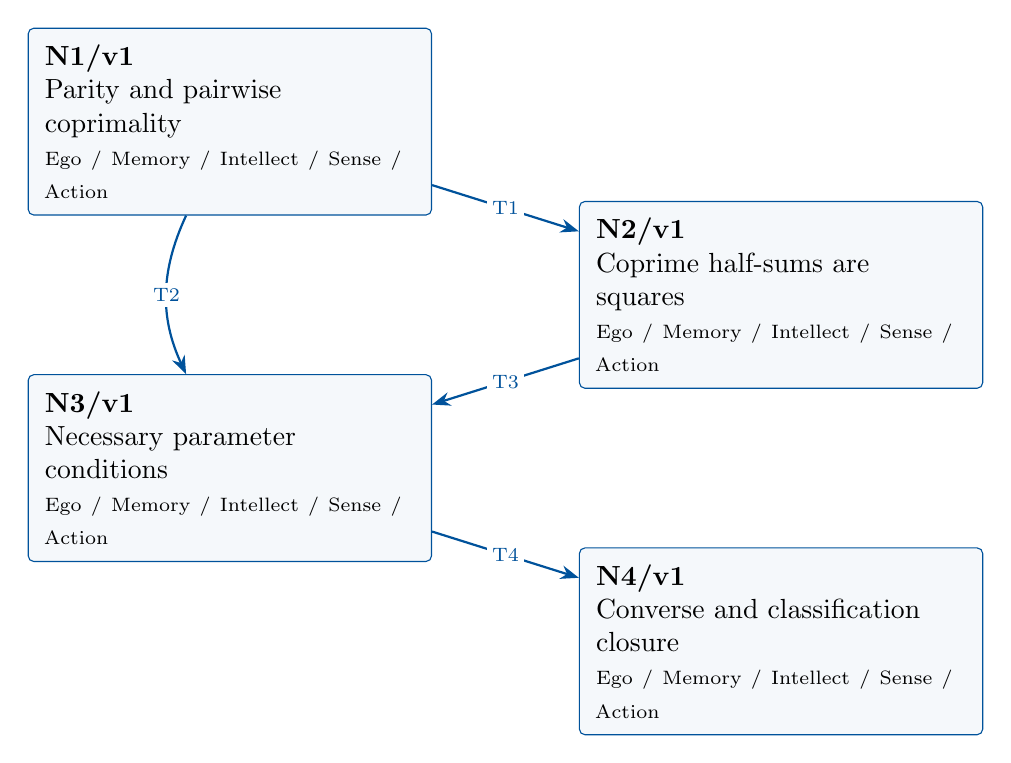
\begin{tikzpicture}[>=Stealth,x=1cm,y=1cm]

\node[mmnode,text width=4.7cm,minimum height=1.35cm] (N1) at (0,0) {\textbf{N1/v1}\\Parity and pairwise coprimality\\{\scriptsize Ego / Memory / Intellect / Sense / Action}};

\node[mmnode,text width=4.7cm,minimum height=1.35cm] (N2) at (7,-2.2) {\textbf{N2/v1}\\Coprime half-sums are squares\\{\scriptsize Ego / Memory / Intellect / Sense / Action}};

\node[mmnode,text width=4.7cm,minimum height=1.35cm] (N3) at (0,-4.4) {\textbf{N3/v1}\\Necessary parameter conditions\\{\scriptsize Ego / Memory / Intellect / Sense / Action}};

\node[mmnode,text width=4.7cm,minimum height=1.35cm] (N4) at (7,-6.6) {\textbf{N4/v1}\\Converse and classification closure\\{\scriptsize Ego / Memory / Intellect / Sense / Action}};

\draw[mmproof] (N1) to node[mmnote,pos=.5] {T1} (N2);

\draw[mmproof,bend right=25] (N1) to node[mmnote,pos=.5] {T2} (N3);

\draw[mmproof] (N2) to node[mmnote,pos=.5] {T3} (N3);

\draw[mmproof] (N3) to node[mmnote,pos=.5] {T4} (N4);

\end{tikzpicture}\end{center}

\reportcaption{Blue arrows are accepted mathematical dependencies, with exact transfers T1--T4 below. Repair messages are described separately; they are not premises of the proof.}

\subsection{Versioned evidence-transfer ledger}

\begingroup\small\linespread{1.05}\selectfont\renewcommand{\field}[2]{\par\noindent\textbf{#1.} #2\par}

\Needspace{5\baselineskip}\smallskip\noindent\textbf{T1: N1/E1 v1 to N2.1–2}

\field{Claim}{After exchanging legs, \(b\) is even, \(a,c\) are odd, and every pair
among \(a,b,c\) is coprime.}

\field{Compatibility}{Odd half-sums are integral and the required pairwise gcd is one.}

\field{Evidence}{Node N1 activities below and the continuous proof in Section~\ref{sec:proof}.}

\Needspace{5\baselineskip}\smallskip\noindent\textbf{T2: N1/E1 v1 to N3.3}

\field{Claim}{After exchanging legs, \(b\) is even, \(a,c\) are odd, and every pair
among \(a,b,c\) is coprime.}

\field{Compatibility}{The recovered odd leg and hypotenuse constrain parameter parity.}

\field{Evidence}{Node N1 activities below and the continuous proof in Section~\ref{sec:proof}.}

\Needspace{5\baselineskip}\smallskip\noindent\textbf{T3: N2/E2 v1 to N3.1–2}

\field{Claim}{For \(u=(c+a)/2\), \(v=(c-a)/2\), one has \(u=m^2\), \(v=n^2\) for
coprime integers \(m>n\ge1\).}

\field{Compatibility}{Use positive integer square roots with their order and gcd.}

\field{Evidence}{Node N2 activities below and the continuous proof in Section~\ref{sec:proof}.}

\Needspace{5\baselineskip}\smallskip\noindent\textbf{T4: N3/E3 v1 to N4.3}

\field{Claim}{Every primitive triple has \(a=m^2-n^2\), \(b=2mn\), \(c=m^2+n^2\), with
\(m>n\ge1\), coprime and of opposite parity.}

\field{Compatibility}{N3 supplies only the forward half; N4 proves the converse independently
before joining.}

\field{Evidence}{Node N3 activities below and the continuous proof in Section~\ref{sec:proof}.}

\endgroup

\clearpage\section{Agent roles and five-faculty activities}

\subsection{N1/v1: Parity and pairwise coprimality}

\field{Object and role}{Choose a consistent leg orientation and prove the arithmetic constraints
needed for half-sums.}

\field{Inputs}{A positive primitive triple \(a^2+b^2=c^2\); prime-divisor facts.}

\mmfaculty{E}{Ego}{Publish the orientation and pairwise gcd facts, not just collective
primitiveness.}

\mmfaculty{M}{Memory}{Retain square residues modulo \(4\) and
\(p\mid x^2\Rightarrow p\mid x\).}

\mmfaculty{I}{Intellect}{Exclude both-even and both-odd legs; transfer a shared prime through the
equation.}

\mmfaculty{S}{Sense}{Renaming the legs is allowed; a common divisor must be ruled out for
each pair.}

\mmfaculty{A}{Action}{Both even legs would make \(c\) even, contradicting primitiveness.
Continue with the numbered deductions below, retaining the exact export.}

\smallskip\noindent\textbf{Numbered mathematical activities}

\begin{enumerate}[label=N1.\arabic*,leftmargin=3.4em]

\item Both even legs would make \(c\) even, contradicting primitiveness.

\item Both odd legs give \(c^2\equiv2\pmod4\), impossible; rename the even leg
\(b\).

\item Then \(a,c\) are odd. A prime dividing two entries divides the square,
and hence the value, of the third; all pairs are coprime.

\end{enumerate}

\field{Export E1/v1}{After exchanging legs, \(b\) is even, \(a,c\) are odd, and every pair
among \(a,b,c\) is coprime.}

\field{Acceptance gate}{Parity and all three pairwise gcd conclusions follow from the original
primitive-triple hypothesis.}

\field{Targeted repair}{If the input is not primitive, stop this classification or explicitly
divide out the common factor under a new task; recheck N2 and N3.}

\clearpage

\subsection{N2/v1: Coprime half-sums are squares}

\field{Object and role}{Extract integer parameters from a square product with disjoint prime
support.}

\field{Inputs}{N1/E1 and NT-02 unique prime factorization.}

\mmfaculty{E}{Ego}{Publish integer square parameters only after positivity, integrality,
and coprimality are proved.}

\mmfaculty{M}{Memory}{Retain \(a,c\) odd, \(c>a>0\), and \(\gcd(a,c)=1\).}

\mmfaculty{I}{Intellect}{Use half-sums to produce coprime factors whose product is a square.}

\mmfaculty{S}{Sense}{A square product alone is insufficient: \(2\cdot8=16\) with neither
factor square.}

\mmfaculty{A}{Action}{Set \(u=(c+a)/2\), \(v=(c-a)/2\). Then \(u>v>0\) are integers and
\(uv=(b/2)^2\). Continue with the numbered deductions below, retaining
the exact export.}

\smallskip\noindent\textbf{Numbered mathematical activities}

\begin{enumerate}[label=N2.\arabic*,leftmargin=3.4em]

\item Set \(u=(c+a)/2\), \(v=(c-a)/2\). Then \(u>v>0\) are integers and
\(uv=(b/2)^2\).

\item A positive common divisor of \(u,v\) divides \(u+v=c\) and \(u-v=a\), so
it is \(1\).

\item Unique factorization gives even prime exponents in each disjoint factor;
take positive square roots \(u=m^2\), \(v=n^2\).

\end{enumerate}

\field{Export E2/v1}{For \(u=(c+a)/2\), \(v=(c-a)/2\), one has \(u=m^2\), \(v=n^2\) for
coprime integers \(m>n\ge1\).}

\field{Acceptance gate}{The square roots are positive integers and \(\gcd(m,n)=1\), since any
common prime would divide \(u,v\).}

\field{Targeted repair}{Restore the coprimality proof before splitting the square product;
invalidate N3 and the classification assembly in N4.}

\clearpage

\subsection{N3/v1: Necessary parameter conditions}

\field{Object and role}{Recover all three entries and enforce the parameter parity restriction.}

\field{Inputs}{N1/E1 and N2/E2.}

\mmfaculty{E}{Ego}{Publish the full parameter contract, including parity and the chosen leg
orientation.}

\mmfaculty{M}{Memory}{Retain the half-sum equations and the positivity of \(b,m,n\).}

\mmfaculty{I}{Intellect}{Recombine sums and differences and choose the positive square root for
the even leg.}

\mmfaculty{S}{Sense}{The polynomial identity alone does not imply primitiveness or opposite
parity.}

\mmfaculty{A}{Action}{From \(u=m^2,v=n^2\), obtain \(a=u-v\) and \(c=u+v\). Continue with the
numbered deductions below, retaining the exact export.}

\smallskip\noindent\textbf{Numbered mathematical activities}

\begin{enumerate}[label=N3.\arabic*,leftmargin=3.4em]

\item From \(u=m^2,v=n^2\), obtain \(a=u-v\) and \(c=u+v\).

\item Because \((b/2)^2=m^2n^2\) and all terms are positive, \(b=2mn\).

\item Both parameters even contradict coprimality; both odd would make \(a,c\)
even. They have opposite parity.

\end{enumerate}

\field{Export E3/v1}{Every primitive triple has \(a=m^2-n^2\), \(b=2mn\), \(c=m^2+n^2\), with
\(m>n\ge1\), coprime and of opposite parity.}

\field{Acceptance gate}{All displayed formulas and every parameter condition are derived,
without guessing a square-root sign.}

\field{Targeted repair}{If a parameter condition is missing, withhold the forward classification
and recheck its use in N4.}

\clearpage

\subsection{N4/v1: Converse and classification closure}

\field{Object and role}{Prove that admissible parameters generate primitive triples, then join
both directions.}

\field{Inputs}{Fresh parameters \(m>n\ge1\), coprime and opposite parity; N3/E3 for the
forward direction.}

\mmfaculty{E}{Ego}{Publish a classification only after both the forward construction and
converse are established.}

\mmfaculty{M}{Memory}{Retain Euclid's lemma, opposite parity, and the parameter gcd; keep the
converse independent of assuming a primitive output.}

\mmfaculty{I}{Intellect}{Expand the identity and rule out common prime divisors of the two
constructed legs.}

\mmfaculty{S}{Sense}{An identity check alone misses nonprimitive triples; treat the prime
\(2\) separately.}

\mmfaculty{A}{Action}{Expand \((m^2-n^2)^2+(2mn)^2=(m^2+n^2)^2\); positivity follows from
\(m>n\ge1\). Continue with the numbered deductions below, retaining the
exact export.}

\smallskip\noindent\textbf{Numbered mathematical activities}

\begin{enumerate}[label=N4.\arabic*,leftmargin=3.4em]

\item Expand \((m^2-n^2)^2+(2mn)^2=(m^2+n^2)^2\); positivity follows from
\(m>n\ge1\).

\item An odd prime dividing both legs divides \(m\) or \(n\), and then the
other, contradicting coprimality.

\item The leg \(m^2-n^2\) is odd, excluding the common prime \(2\). Thus the
legs, and hence the triple, are primitive; join N3's forward direction.

\end{enumerate}

\field{Export E4/v1}{Exactly the primitive positive triples, up to exchanging legs, arise
from the stated formulas.}

\field{Acceptance gate}{Identity, positivity, and absence of every common prime are proved for
arbitrary admissible parameters.}

\field{Targeted repair}{If both parameters are odd, reject the input under this contract; do not
publish a nonprimitive example as a primitive triple.}

\clearpage\section{Continuous mathematical proof}\label{sec:proof}

\begin{proof}

Let \((a,b,c)\) be a positive primitive triple. If both legs were even,
the equation would make \(c\) even. If both were odd, their squared sum
would be \(2\) modulo \(4\), impossible for a square. Hence exactly one
leg is even; call it \(b\). Then \(a,c\) are odd. If a prime divided two
entries, the equation would make it divide the square of the third, and
Euclid's lemma would make it divide the third entry too. This
contradicts primitiveness. Thus all pairs are coprime (N1).

Since \(c^2=a^2+b^2>a^2\), positivity gives \(c>a\). Define
\[u=\frac{c+a}{2},\qquad v=\frac{c-a}{2}.\] These are integers with
\(u>v>0\) and \(uv=(b/2)^2\). A positive common divisor of \(u,v\)
divides \(c=u+v\) and \(a=u-v\), so \(\gcd(u,v)=1\). Every prime occurs
in at most one of their factorizations. Since the product is a square,
uniqueness of factorization forces each exponent in each factor to be
even, including the empty factorization if a factor is \(1\). Therefore
\(u=m^2\), \(v=n^2\) for positive integers \(m>n\). A common prime of
\(m,n\) would divide \(u,v\), so \(\gcd(m,n)=1\) (N2).

It follows that \(a=m^2-n^2\), \(c=m^2+n^2\), and, taking the positive
square root of \((b/2)^2=m^2n^2\), \(b=2mn\). The parameters cannot both
be even by coprimality, or both odd because \(a,c\) are odd. Thus they
have opposite parity (N3).

Conversely, take any parameters meeting these conditions (N4). The
formulas give positive integers, and direct expansion gives the
Pythagorean equation. If an odd prime \(p\) divided both \(m^2-n^2\) and
\(2mn\), Euclid's lemma would give \(p\mid m\) or \(p\mid n\). Either
case, together with \(p\mid m^2-n^2\), implies that \(p\) divides the
square and then the value of the other parameter, contradicting their
gcd. The prime \(2\) cannot divide both legs, because opposite parity
makes \(m^2-n^2\) odd. Any common divisor greater than \(1\) would have
a prime divisor, so the two legs are coprime and the triple is
primitive. Both directions prove the classification. The parameters are
also recoverable uniquely after choosing the even leg, as
\(m=\sqrt{(c+a)/2}\) and \(n=\sqrt{(c-a)/2}\).

\end{proof}

\section{Worked orchestration}

Start with \((a,b,c)=(5,12,13)\). N1 checks the even leg and pairwise
gcds. N2 obtains \[u=\frac{13+5}{2}=9,\qquad v=\frac{13-5}{2}=4,\] so
\(m=3,n=2\). N3 recovers \(5=9-4\), \(12=2\cdot3\cdot2\), and
\(13=9+4\). The parameters are coprime and of opposite parity.

In the converse direction, \(m=4,n=1\) produces \((15,8,17)\), and
\(15^2+8^2=225+64=289=17^2\). The parameter test and N4's prime-divisor
argument justify primitiveness, beyond the numerical identity.

\subsection{Boundary and hypothesis audit}

\begin{itemize}
\item
  \(m=2,n=1\) gives \((3,4,5)\) and includes the allowed boundary
  \(n=1\). The case \(n=0\) would give a zero leg and is excluded.
\item
  \(m=3,n=1\) gives \((8,6,10)\), showing that coprime parameters with
  the same parity need not give a primitive triple.
\item
  \(m=6,n=3\) gives \((27,36,45)\): opposite parity alone does not imply
  coprimality. Both conditions are enforced. A square product without
  coprimality, such as \(2\cdot8=16\), cannot justify square factors.
\end{itemize}

\section{Illustrative failure and repair}

This is a deliberately authored teaching trace. A diagnostic asks for
correction; it cannot prove a predecessor by importing its descendant's
conclusion. A revised export must be checked before its consumers are
reused.

\field{Candidate}{N2 infers that \(u,v\) are squares from \(uv\) being a square, omitting
the gcd check.}

\field{Detection}{Sense supplies \(u=2,v=8\), for which \(uv=16\) but neither factor is
square.}

\field{Correction}{Memory retrieves \(\gcd(a,c)=1\) from N1. Action proves \(\gcd(u,v)=1\)
via their sum and difference; Intellect then applies disjoint
prime-exponent parity.}

\field{Recheck}{Re-establish N2's integer parameters and N3's formulas and parity.
Recheck the N4 forward/converse assembly.}

\field{Publication}{Ego publishes square splitting only for coprime positive factors. This
fills the missing inference under the original primitive-triple
assumptions.}

\section{Reusable result and provenance}
Reusable exports retain each node's version 1 statement, assumptions, and proof.
The final export is the theorem in Section 1, proved relative to its declared imports.

\smallskip\noindent\textbf{Source record.} Adapted from the original project Markdown:
\par\noindent\nolinkurl{classification-of-primitive-pythagorean-triples.md}\par
Typography, workflow conventions, and faculty cards follow the workspace Meta-Math
manuscript. This authored exposition does not claim formal certification.
\end{document}
